% -------------------------------------------------------------------------------------------------
%      MDSG Latex Framework
%      ============================================================================================
%      File:                  main.tex
%      Author(s):             Michael Duerr
%      Version:               1
%      Creation Date:         30. Mai 2010
%      Creation Date:         30. Mai 2010
%
%      Notes:                 - This represents the document root of this template
%                             - Binding correction is 12mm. In case you change this value, you
%                               may also need to adapt the value of \bcorlength in mdsg.sty
%                             - Switch `babel' package options `english' and `ngerman' in case
%                               your thesis is in English
%                             - if you prefer to use utf8 encoding, uncomment the corresponding
%                               line `\usepackage[utf8]{inputenc}' and comment the line
%                               `\usepackage[latin1]{inputenc}'. To compile this example you also
%                               need to include the corresponding introduction example file i.e.
%                               `introduction-UTF8.tex' or `introduction-ISO8859-1.tex'
% -------------------------------------------------------------------------------------------------
%
\documentclass[bibliography=totoc,listof=totoc,index=totoc,twoside=true,BCOR=12mm,DIV=12]{scrbook}
%\KOMAoptions{draft=true}                         % uncomment if you want to visualise overful hbox
%\KOMAoptions{chapterprefix=true}                 % uncomment if you like "Chapter" in front of
                                                  % chapter number
%\KOMAoptions{appendixprefix=true}                % uncomment if you like "Appendix" in front of
                                                  % appendix number
%\KOMAoptions{...}                                % feel free to add additional KOMA options
%
% =================================================================================================
% set encoding
% -------------------------------------------------------------------------------------------------
%
\usepackage[utf8]{inputenc}                       % uncomment if you prefer utf8 encoding
%\usepackage[latin1]{inputenc}                    % uncomment if you prefer latin1 encoding
%
% =================================================================================================
% load mdsg style
% -------------------------------------------------------------------------------------------------
%
%\usepackage[diplom]{mdsg}                        % uncomment the corresponding option
%\usepackage[fopra]{mdsg}
%\usepackage[bachelor]{mdsg}
\usepackage[master]{mdsg}
%
% =================================================================================================
% initialize macros
% -------------------------------------------------------------------------------------------------
%
\lmutitle{Titel der Arbeit}                       % title: you can force a new line by
%\lmutitle{Titel \\ der \\ Arbeit}                % inserting `\\'. However, this will cause
                                                  % a hyperref warning!
\lmustudentone{Judith Greif}                    	 % first author's name
%\lmustudenttwo{Max2 Mustermann2}                 % second author's name
%\lmustudentthree{Max3 Mustermann3}               % third author's name
%\lmustudentfour{Max4 Mustermann4}                % fourth author's name

\lmuprofone{Prof. Dr. Claudia Linnhoff-Popien}    % first supervisor's name
%\lmuproftwo{Prof. Dr. Max Mustermann}             % second supervisor's name
                                                  % (uncomment if not needed)
%\lmuprofthree{Prof. Dr. Max2 Mustermann2}         % third supervisor's name
                                                  % (uncomment if not needed)
\lmuadvisorone{Mirco Schönfeld}                    % first advisor's name
%\lmuadvisortwo{Betreuer Name2}                    % second advisor's name
                                                  % (uncomment if not needed)
%\lmuadvisorthree{Betreuer Name3}                  % third advisor's name
                                                  % (uncomment if not needed)
\lmudraftdate{\today}                             % only for versioning during work!
                                                  % (uncomment for final version!)
\lmudeadline{1. Januar 2099}                      % deadline (day of submission)
%
% =================================================================================================
% package selection (add additional packages if needed)
% -------------------------------------------------------------------------------------------------
%
%\usepackage{layout}                              % see documentation of this package
\usepackage{cmap}                                 % to produce searchable PDF
\usepackage[T1]{fontenc}                          % split german words with umlaut
\usepackage{lmodern}
\usepackage[english,ngerman]{babel}               % for german toc, ...
\usepackage{bibgerm}                              % for german bibliography index
\usepackage{tabularx}                             % more flexible table environment
\usepackage{booktabs}                             % high quality tables
\usepackage{rotating}                             % for generation of landscape tables
\usepackage{multirow}                             % for multirow cells inside tables
\usepackage{amssymb,amsmath}                      % powerful math package
\usepackage{hyperref}                             % for hyperlinks
\lmuhypersetup                                    % write some pdf properties
\usepackage{flafter}                              % force floats to appear after their reference
\usepackage{subfig}                               % to allow for side by side graphics (subfloats)
\usepackage{pdflscape}                            % enable rotation of landscape pages
\usepackage{hyphenat}                             % proper hyphenation for bla_bla to bla_-bla
\usepackage[all]{hypcap}                          % correct captions
\usepackage{url}                                  % nicer url style
\usepackage{enumitem}                             % for tight lists
\usepackage{textcomp}
%\usepackage{...}                                 % add additional packages here

\setcounter{tocdepth}{3}                          % sectioning depth in toc
\setcounter{secnumdepth}{3}                       % sectioning depth in text

\graphicspath{{./pictures/}}                      % put all graphics here
% -------------------------------------------------------------------------------------------------
%      MDSG Latex Framework
%      ============================================================================================
%      File:                  hyphenation.tex
%      Author(s):             Michael Duerr
%      Version:               1
%      Creation Date:         30. Mai 2010
%      Creation Date:         30. Mai 2010
%
%      Notes:                 - Instruction \hypenation cannot handle special characters like umlaute
%                               as well as  "a and \"a. Split such words in your text.
%
% -------------------------------------------------------------------------------------------------
%
\hyphenation{Ba-che-lor-ar-}
%\hyphenation{...}                           % further hyphenation examples
                               % this file holds words latex cannot split
%
% =================================================================================================
% start of document
% -------------------------------------------------------------------------------------------------
%
\begin{document}
    \setlist{noitemsep}                           % for tight lists
    \lmufront                                     % title pages
    \newpage
    \cleardoublepage
    \lmuaffirmation                               % affirmation (work is my own work)
    \newpage
    \cleardoubleemptypage
    \thispagestyle{empty}
    % -------------------------------------------------------------------------------------------------
%      MDSG Latex Framework
%      ============================================================================================
%      File:                  abstract.tex
%      Author(s):             Michael Duerr
%      Version:               1
%      Creation Date:         30. Mai 2010
%      Creation Date:         30. Mai 2010
%
%      Notes:                 - Place your abstract here
% -------------------------------------------------------------------------------------------------
%
\vspace*{2cm}

\begin{center}
    \textbf{Abstract}
\end{center}

\vspace*{1cm}

\noindent Ubiquitous computing und die Zunahme mobiler Endgeräte haben zu neuen Kommunikationsmustern im Internet geführt: Weg von adressbasiertem Routing und Ende-zu-Ende-Kommunikation hin zu \textit{Information-centric Networking}. Kontextzentrische soziale Netze sind ein Ansatz, dem Rechnung zu tragen. Kommunikation basiert darin nicht auf Online-Freundschaft, sondern allein auf Kontext-Ähnlichkeit. Das kontextzentrische soziale Netz AMBIENCE verwendet Bloom-Filter, um Nachrichten zu kodieren, speichern und anzufragen. Diese müssen so an einem Host organisiert werden, dass die \textit{k} nächsten Nachbarn zu einem Anfragefilter möglichst schnell und effizient gefunden werden. Die vorliegende Arbeit optimiert das mengentheoretische Problem der \textit{k}-nächsten-Nachbarn-Suche für dieses Szenario. Dazu wurde eine Indexstruktur für Bloom-Filter basierend auf einem B$^+$-Baum entwickelt. Die Bloom-Filter werden darin nach ihren Teil- und Obermengenbeziehungen organisiert, der \textit{BloomFilterTree}. Bei der \textit{k}-nächsten-Nachbarn-Suche wird nur der beste Pfad im Baum verfolgt und Teilbäume möglichst früh abgeschnitten. Kriterien für die Evaluation waren Ergebnisqualität, CPU-Zeit, Zeitkomplexität, Speicherbedarf und Aufbaukosten. Im verwendeten Versuchsaufbau ließen sich Zeitkomplexität und CPU-Zeit der \textit{k}-nächste-Nachbarn-Suche mit dem BloomFilterTree um bis zu 68\% bzw. 87\% reduzieren.                        % abstract
    \thispagestyle{empty}
    \frontmatter                                  % start roman numbering
    \tableofcontents                              % toc
    \mainmatter                                   % start alpha numbering
%
% =================================================================================================
% place your document text here (take care of encoding)
% -------------------------------------------------------------------------------------------------
%
    %% -------------------------------------------------------------------------------------------------
%      MDSG Latex Framework
%      ============================================================================================
%      File:                  introduction-[UTF8,ISO8859-1].tex
%      Author(s):             Michael Duerr
%      Version:               1
%      Creation Date:         30. Mai 2010
%      Creation Date:         30. Mai 2010
%
%      Notes:                 - Example chapter
% -------------------------------------------------------------------------------------------------
%
\chapter{Einleitung}\label{sec:Introduction}
Dies ist der \LaTeX\ Rahmen zur Bearbeitung von Bachelor-, Master-, Projekt- und Diplomarbeiten.
Alle relevanten Dateien befinden sich im Verzeichnis \verb|text|.
\section{Unterverzeichnisse und Dateien}
Das Verzeichnis \verb|text| beinhaltet weitere Unterverzeichnisse und Dateien, die den Rahmen charakterisieren.
\subsection{\textbf{main.tex}}\label{subsec:main}
Diese Datei stellt die zentrale Konfigurationsdatei für den Rahmen dar. Unter anderem müssen hier Informationen
über die Aufgabensteller, Betreuer, die Art der Arbeit sowie deren Title eingestellt werden.
Hier können auch weitere Pakete eingebunden werden. Die Datei ist dokumentiert und sollte selbsterklärend
sein.
\subsection{\textbf{hyphenation.tex}}
Manche Wörter werden von \LaTeX\ nicht (ordentlich) getrennt. Diese können in dieser Datei mit deren
Trennungsstellen hinzugefügt werden.
\subsection{\textbf{Makefile}}
Um das Dokument zu erstellen muss man den Aufruf \verb|make all| tätigen. Dabei werden einige temporäre
Dateien erstellt sowie die Datei \verb|main.pdf| die das entsprechende Dokument enthält. Mir dem
Aufruf \verb|make clean| werden alle temporären Dateien sowie die Datei \verb|main.pdf| gelöscht.
sie können die Datei \verb|Makefile| ihren Anforderungen entsprechend erweitern.
\subsection{\textbf{text}}
Es bietet sich an für verschiedene Kapitel eigene Quelldateien zu pflegen. Diese sollten sie alle im
Ordner \verb|text| ablegen. Wie ein Kapitel eingebunden wird, kann man aus dem Beispiel in der
Datei \verb|main.tex| ablesen. Das Verzeichnis \textbf{text} beinhaltet zudem die Datei
\verb|abstract.tex|. In diese Datei soll eine kurze Zusammenfassung (ca. eine halbe Seite)
der Arbeit eingetragen werden. Die Datei \verb|appendix.tex| kann verwendet werden um einen
Anhang zu generieren.
\subsection{\textbf{pictures}}
Hier müssen sie alle Grafiken ablegen, die sie in ihrem Dokument einbinden wollen. Es sind nur die
Formate PDF, PNG und JPEG erlaubt (GIF ist möglich, wird aber nicht empfohlen).
\subsection{\textbf{bibliography.bib}}
In diese Datei müssen alle Referenzen eingetragen werden,
die innerhalb ihrer Arbeit zitiert werden. Verwenden sie zur Verwaltung ihrer Referenzen einen
geeigneten Editor z.B. \textit{JabRef} (\url{http://jabref.sourceforge.net/}).
\subsection{\textbf{mdsg.sty}}
Hierbei handelt es sich um das Stylefile, das das Erscheinungsbild des Dokuments
lenkt. In dieser Datei sollten in der Regel keine Veränderungen notwendig sein.
\section{Beispiele}
Es gibt eine Unmenge an \LaTeX\ Tutorials und Dokumentationen, die guten Einstieg in das Arbeiten mit
\LaTeX\ ermöglichen. Im Folgenden werden aber ein paar undokumentierte Minimalbeispiele gegeben, die
den direkten Einstieg ermöglichen. Betrachten sie den Quelltext, um die Beispiele nachzuvollziehen.
\subsection{Zitate}
Wir zitieren hier eine Quelle von James Aspnes et al \cite{aspn07}, die in der  Datei\\
\verb|bibliography.bib|
steht.
\subsection{Listen}
Es gibt verschiedene Möglichkeiten Listen zu erstellen, z.B. ohne Nummerierung\dots
\begin{itemize}
   \item
      Das ist der erste Punkt,
      \begin{itemize}
         \item
            das der erste Unterpunkt,
         \item
            das der zweite Unterpunkt,
   \end{itemize}
   \item
      das der zweite, und
   \item
      das der dritte Punkt.
\end{itemize}
\dots oder mit Nummerierung\dots
\begin{enumerate}
   \item
      Das ist der erste Punkt,
      \begin{enumerate}
         \item
            das der erste Unterpunkt,
         \item
            das der zweite Unterpunkt,
      \end{enumerate}
   \item
      das der zweite, und
   \item
      das der dritte Punkt.
\end{enumerate}
\subsection{Referenz auf anderen Text}
Es ist auch möglich auf andere Stellen im Text z.B. Kapitel \ref{subsec:main} zu verweisen.
\subsection{Hoch- und tiefgestellter Text}
Man kann Text tiefstellen indem man \verb|\textsubscript| verwendet, z.B. ergibt
\begin{verbatim}
text\textsubscript{tiefgestellt}
\end{verbatim}
den Text text\textsubscript{tiefgestellt}.
Das selbe funktioniert mit \verb|\textsuperscript| verwendet, z.B. ergibt
\begin{verbatim}
text\textsuperscript{hochgestellt}
\end{verbatim}
text\textsuperscript{hochgestellt}
\subsection{Tabellen}
Es gibt schöne Möglichkeiten Tabellen einzubinden wie z.B. Tabelle \ref{tab:CommonParameterSettings}.
\begin{center}
\begin{table}[htbp]
{\small
\begin{center}
\begin{tabular}[center]{lrlc}
\toprule
Parameter & Value & (Unit) & Available for Chord \\
\midrule
Query timeout & 10 & seconds & $\surd$ \\
Republish timeout & 300 & seconds & $\surd$ \\ % explain this value...
Stabilize timeout & 5 & seconds & $\surd$ \\
Fix fingers timeout & 30 & seconds & $\surd$ \\
Message timeout & 1 & second & $\surd$ \\
Connect timeout & 10 & seconds & $\surd$ \\
Ping superpeer timeout & 5 & seconds & $\times$ \\
Cost-Optimality estimation timeout & 20 & seconds & $\times$ \\
Significance for change in number of superpeers & 10 & percent & $\times$ \\
Significance for change in estimations  & 10 & percent & $\times$ \\
Number of permanent superpeers & 32 & nodes & $\times$ \\
Mean number of peers & 1000 & nodes & $\surd$ \\
Mean number of lookups per hour & 60 & queries & $\surd$ \\
Mean number of shared InfoProfiles per node & 20 & & $\surd$ \\
Identifier space & 16 & bits & $\surd$ \\
Direct insertion acknowledgment & true & bool & $\times$ \\
Direct query responses & true & bool & $\times$ \\
Force query resolution & true & bool & $\surd$  \\
\bottomrule
\end{tabular}
\end{center}
} % end of tiny
\caption[Simulation parameter settings]{Common simulation parameter settings.\label{tab:CommonParameterSettings}}
\end{table}
\end{center}

\subsection{Bilder}
Man kann sehr einfach Bilder einbinden so wie z.B. in Abbildung \ref{fig:pic0}.
\begin{figure}[hpbt]
  \centering
  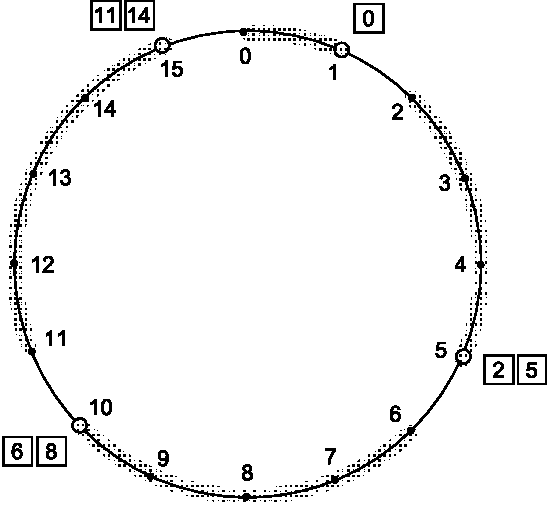
\includegraphics[width=0.4\textwidth]{pictures/pic0}\\
  \caption[Example of a $4$-bit Chord identifier circle]{Example of a $4$-bit Chord identifier circle.
  The responsibility ranges for each peer are accentuated in light gray}\label{fig:pic0}
\end{figure}
Es lassen sich auch mehrere Bilder nebeneinander platzieren wie z.B. in Abbildung
\ref{fig:multipic} zu sehen ist.
\begin{figure}[hpbt]
 \centering
  %%----start of first subfigure----
  \subfloat[FIFO size limited to 20 entries]{
   \label{fig:multipic:a} %% label for first subfigure
   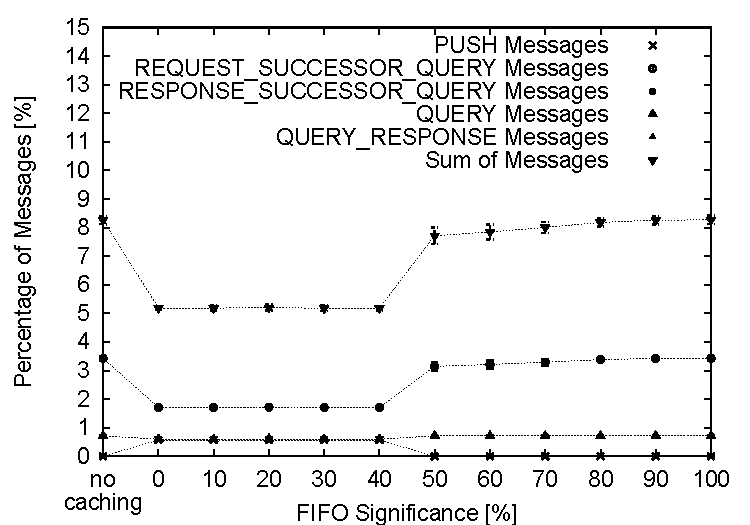
\includegraphics[width=0.48\linewidth]{pic1}}
  \hspace{0.01\textwidth}
  %%----start of second subfigure----
  \subfloat[FIFO size limited to 30 entries]{
   \label{fig:multipic:b} %% label for second subfigure
   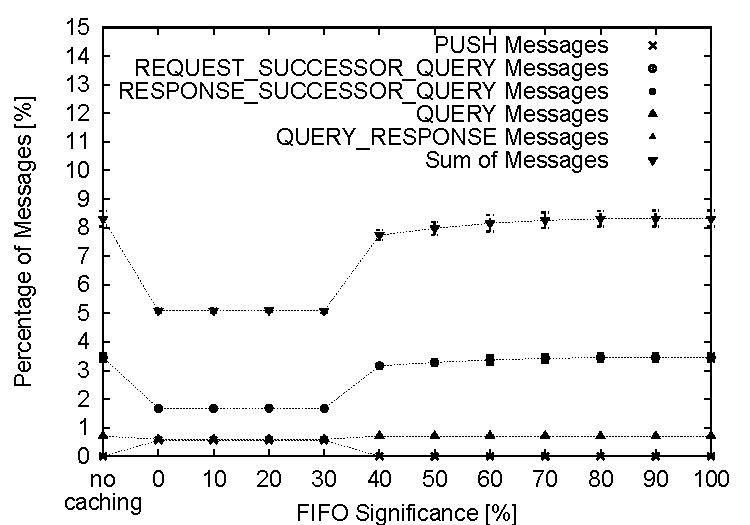
\includegraphics[width=0.48\linewidth]{pic2}}\\[0pt] % horizontal break
  %%----start of third subfigure----
  \subfloat[FIFO size limited to 40 entries]{
   \label{fig:multipic:c} %% label for third subfigure
   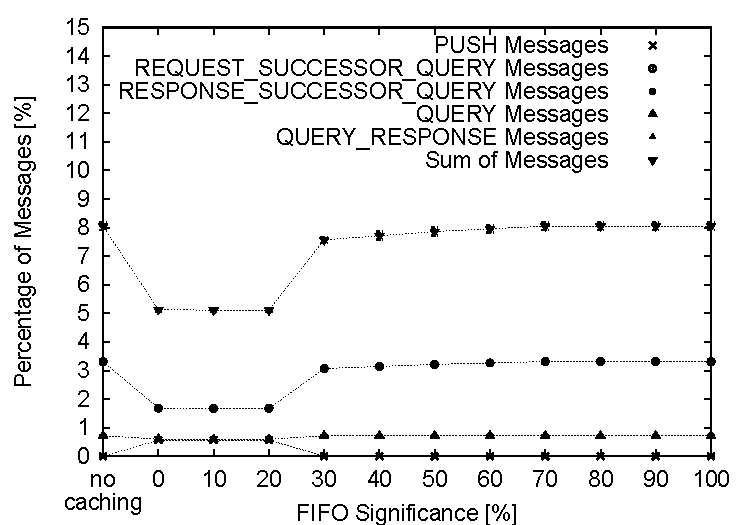
\includegraphics[width=0.48\linewidth]{pic3}}
  \hspace{0.01\textwidth}
  %%----start of fourth subfigure----
  \subfloat[FIFO size limited to 50 entries]{
   \label{fig:multipic:d} %% label for fourth subfigure
   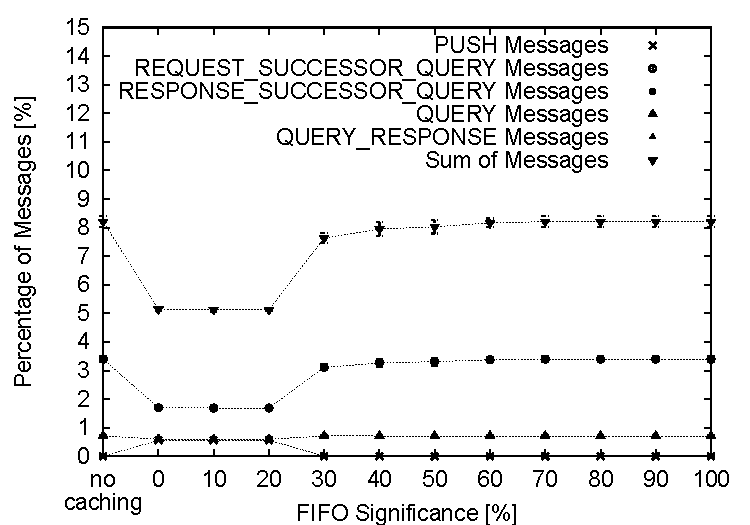
\includegraphics[width=0.48\linewidth]{pic4}}
 \caption[Observed message fractions and 95\% confidence intervals for Chord]{Observed message fractions and 95\% confidence intervals for Chord without the influence of churn. The FIFO capacity varies from 20 (\ref{fig:multipic:a}) -- 50 (\ref{fig:multipic:d}) entries (decadic steps).}
 \label{fig:multipic} %% label for entire figure
\end{figure}

\subsection{Programm Code}
Eine elegante Möglichkeit, Programmtext einzubinden, lässt sich mit dem listings-Paket erreichen.
Das \verb|HelloWorld| Programm aus Listing \ref{lst:hw} hat in Zeile \ref{line:hw3} übrigens einen Programmierfehler.
\begin{lstlisting}[float=htp,caption=Hello World,label=lst:hw,language=Java, numbers=left, numberstyle=\tiny, stepnumber=2, numbersep=8pt, escapeinside={//@}{@//},backgroundcolor=\color{yellow},xleftmargin=3ex,xrightmargin=1ex]
public class HelloWorld {
    public static void main(String[] args) {
        Syste.out.println("Hello, World"); //@\label{line:hw3}@//
    }
}
\end{lstlisting}

\subsection{Fußnoten}
Wenn man auf Google \footnote{\url{http://www.google.com}} verweisen will, bietet sich statt einer gesonderten
Referenz auch einfach eine Fußnote an.
\subsection{Formeln}
Man kann mit \LaTeX\ sehr schön Formeln erzeugen:
$$L_{P}(k) = R^{orig}_{P}(k) + \sum_{i=0}^n 2*R^{i}_{P}(k)$$

    %% -------------------------------------------------------------------------------------------------
%      MDSG Latex Framework
%      ============================================================================================
%      File:                  introduction-[UTF8,ISO8859-1].tex
%      Author(s):             Michael Duerr
%      Version:               1
%      Creation Date:         30. Mai 2010
%      Creation Date:         30. Mai 2010
%
%      Notes:                 - Example chapter
% -------------------------------------------------------------------------------------------------
%
\chapter{Einleitung}\label{sec:Introduction}
Dies ist der \LaTeX\ Rahmen zur Bearbeitung von Bachelor-, Master-, Projekt- und Diplomarbeiten.
Alle relevanten Dateien befinden sich im Verzeichnis \verb|text|.
\section{Unterverzeichnisse und Dateien}
Das Verzeichnis \verb|text| beinhaltet weitere Unterverzeichnisse und Dateien, die den Rahmen charakterisieren.
\subsection{\textbf{main.tex}}\label{subsec:main}
Diese Datei stellt die zentrale Konfigurationsdatei f�r den Rahmen dar. Unter anderem m�ssen hier Informationen
�ber die Aufgabensteller, Betreuer, die Art der Arbeit sowie deren Title eingestellt werden.
Hier k�nnen auch weitere Pakete eingebunden werden. Die Datei ist dokumentiert und sollte selbsterkl�rend
sein.
\subsection{\textbf{hyphenation.tex}}
Manche W�rter werden von \LaTeX\ nicht (ordentlich) getrennt. Diese k�nnen in dieser Datei mit deren
Trennungsstellen hinzugef�gt werden.
\subsection{\textbf{Makefile}}
Um das Dokument zu erstellen muss man den Aufruf \verb|make all| t�tigen. Dabei werden einige tempor�re
Dateien erstellt sowie die Datei \verb|main.pdf| die das entsprechende Dokument enth�lt. Mir dem
Aufruf \verb|make clean| werden alle tempor�ren Dateien sowie die Datei \verb|main.pdf| gel�scht.
sie k�nnen die Datei \verb|Makefile| ihren Anforderungen entsprechend erweitern.
\subsection{\textbf{text}}
Es bietet sich an f�r verschiedene Kapitel eigene Quelldateien zu pflegen. Diese sollten sie alle im
Ordner \verb|text| ablegen. Wie ein Kapitel eingebunden wird, kann man aus dem Beispiel in der
Datei \verb|main.tex| ablesen. Das Verzeichnis \textbf{text} beinhaltet zudem die Datei
\verb|abstract.tex|. In diese Datei soll eine kurze Zusammenfassung (ca. eine halbe Seite)
der Arbeit eingetragen werden. Die Datei \verb|appendix.tex| kann verwendet werden um einen
Anhang zu generieren.
\subsection{\textbf{pictures}}
Hier m�ssen sie alle Grafiken ablegen, die sie in ihrem Dokument einbinden wollen. Es sind nur die
Formate PDF, PNG und JPEG erlaubt (GIF ist m�glich, wird aber nicht empfohlen).
\subsection{\textbf{bibliography.bib}}
In diese Datei m�ssen alle Referenzen eingetragen werden,
die innerhalb ihrer Arbeit zitiert werden. Verwenden sie zur Verwaltung ihrer Referenzen einen
geeigneten Editor z.B. \textit{JabRef} (\url{http://jabref.sourceforge.net/}).
\subsection{\textbf{mdsg.sty}}
Hierbei handelt es sich um das Stylefile, das das Erscheinungsbild des Dokuments
lenkt. In dieser Datei sollten in der Regel keine Ver�nderungen notwendig sein.
\section{Beispiele}
Es gibt eine Unmenge an \LaTeX\ Tutorials und Dokumentationen, die guten Einstieg in das Arbeiten mit
\LaTeX\ erm�glichen. Im Folgenden werden aber ein paar undokumentierte Minimalbeispiele gegeben, die
den direkten Einstieg erm�glichen. Betrachten sie den Quelltext, um die Beispiele nachzuvollziehen.
\subsection{Zitate}
Wir zitieren hier die Quellen \cite{Dargie2010}, \cite{Eisenhardt2004}, \cite{Mishra2013}, \cite{Perera2014}, \cite{Qiao2014}, \cite{Rizia2012}, \cite{Sakuma2011}, \cite{Schoenfeld2014}, \cite{Schnell2013}, \cite{Shiraki2009}, \cite{Werner2015}, \cite{Yu2012}, \cite{Zhang2012}, und \cite{Zinsmaier2010}, die in der  Datei\\
\verb|bibliography.bib|
stehen.
\subsection{Listen}
Es gibt verschiedene M�glichkeiten Listen zu erstellen, z.B. ohne Nummerierung\dots
\begin{itemize}
   \item
      Das ist der erste Punkt,
      \begin{itemize}
         \item
            das der erste Unterpunkt,
         \item
            das der zweite Unterpunkt,
   \end{itemize}
   \item
      das der zweite, und
   \item
      das der dritte Punkt.
\end{itemize}
\dots oder mit Nummerierung\dots
\begin{enumerate}
   \item
      Das ist der erste Punkt,
      \begin{enumerate}
         \item
            das der erste Unterpunkt,
         \item
            das der zweite Unterpunkt,
      \end{enumerate}
   \item
      das der zweite, und
   \item
      das der dritte Punkt.
\end{enumerate}
\subsection{Referenz auf anderen Text}
Es ist auch m�glich auf andere Stellen im Text z.B. Kapitel \ref{subsec:main} zu verweisen.
\subsection{Hoch- und tiefgestellter Text}
Man kann Text tiefstellen indem man \verb|\textsubscript| verwendet, z.B. ergibt
\begin{verbatim}
text\textsubscript{tiefgestellt}
\end{verbatim}
den Text text\textsubscript{tiefgestellt}.
Das selbe funktioniert mit \verb|\textsuperscript| verwendet, z.B. ergibt
\begin{verbatim}
text\textsuperscript{hochgestellt}
\end{verbatim}
text\textsuperscript{hochgestellt}
\subsection{Tabellen}
Es gibt sch�ne M�glichkeiten Tabellen einzubinden wie z.B. Tabelle \ref{tab:CommonParameterSettings}.
\begin{center}
\begin{table}[htbp]
{\small
\begin{center}
\begin{tabular}[center]{lrlc}
\toprule
Parameter & Value & (Unit) & Available for Chord \\
\midrule
Query timeout & 10 & seconds & $\surd$ \\
Republish timeout & 300 & seconds & $\surd$ \\ % explain this value...
Stabilize timeout & 5 & seconds & $\surd$ \\
Fix fingers timeout & 30 & seconds & $\surd$ \\
Message timeout & 1 & second & $\surd$ \\
Connect timeout & 10 & seconds & $\surd$ \\
Ping superpeer timeout & 5 & seconds & $\times$ \\
Cost-Optimality estimation timeout & 20 & seconds & $\times$ \\
Significance for change in number of superpeers & 10 & percent & $\times$ \\
Significance for change in estimations  & 10 & percent & $\times$ \\
Number of permanent superpeers & 32 & nodes & $\times$ \\
Mean number of peers & 1000 & nodes & $\surd$ \\
Mean number of lookups per hour & 60 & queries & $\surd$ \\
Mean number of shared InfoProfiles per node & 20 & & $\surd$ \\
Identifier space & 16 & bits & $\surd$ \\
Direct insertion acknowledgment & true & bool & $\times$ \\
Direct query responses & true & bool & $\times$ \\
Force query resolution & true & bool & $\surd$  \\
\bottomrule
\end{tabular}
\end{center}
} % end of tiny
\caption[Simulation parameter settings]{Common simulation parameter settings.\label{tab:CommonParameterSettings}}
\end{table}
\end{center}

\subsection{Bilder}
Man kann sehr einfach Bilder einbinden so wie z.B. in Abbildung \ref{fig:pic0}.
\begin{figure}[hpbt]
  \centering
  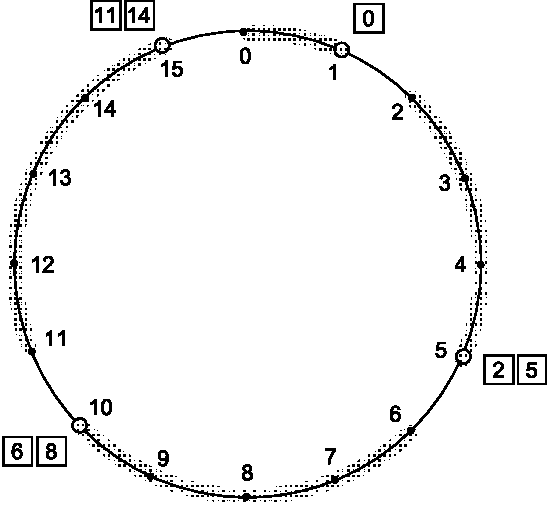
\includegraphics[width=0.4\textwidth]{pictures/pic0}\\
  \caption[Example of a $4$-bit Chord identifier circle]{Example of a $4$-bit Chord identifier circle.
  The responsibility ranges for each peer are accentuated in light gray}\label{fig:pic0}
\end{figure}
Es lassen sich auch mehrere Bilder nebeneinander platzieren wie z.B. in Abbildung
\ref{fig:multipic} zu sehen ist.
\begin{figure}[hpbt]
 \centering
  %%----start of first subfigure----
  \subfloat[FIFO size limited to 20 entries]{
   \label{fig:multipic:a} %% label for first subfigure
   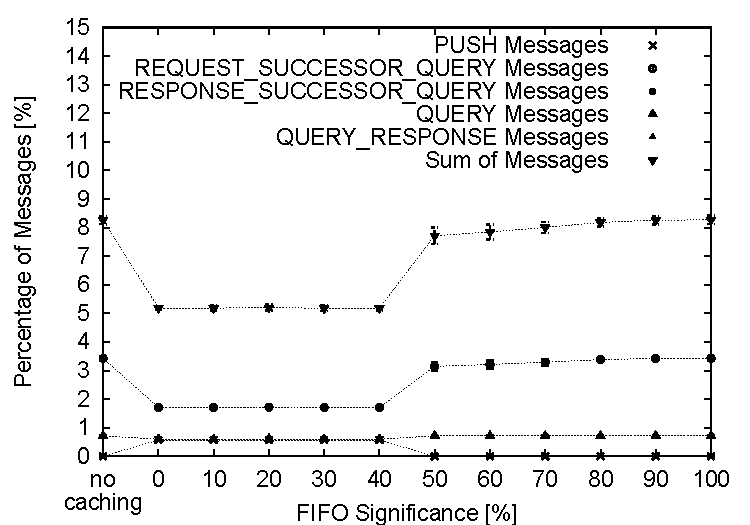
\includegraphics[width=0.48\linewidth]{pic1}}
  \hspace{0.01\textwidth}
  %%----start of second subfigure----
  \subfloat[FIFO size limited to 30 entries]{
   \label{fig:multipic:b} %% label for second subfigure
   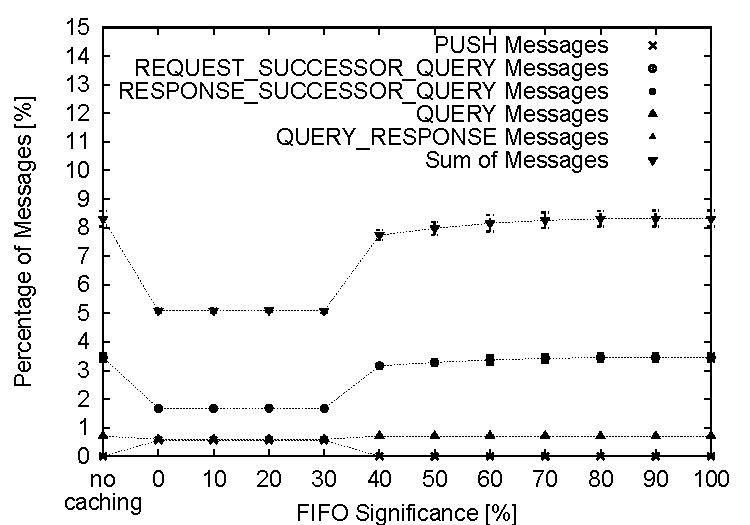
\includegraphics[width=0.48\linewidth]{pic2}}\\[0pt] % horizontal break
  %%----start of third subfigure----
  \subfloat[FIFO size limited to 40 entries]{
   \label{fig:multipic:c} %% label for third subfigure
   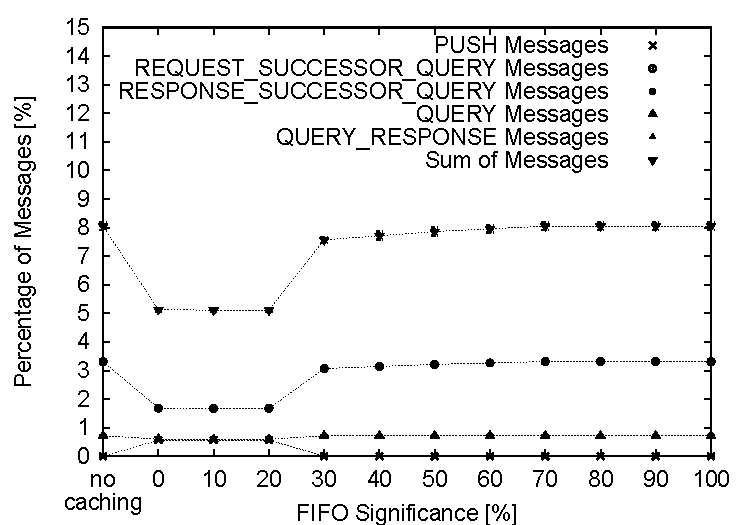
\includegraphics[width=0.48\linewidth]{pic3}}
  \hspace{0.01\textwidth}
  %%----start of fourth subfigure----
  \subfloat[FIFO size limited to 50 entries]{
   \label{fig:multipic:d} %% label for fourth subfigure
   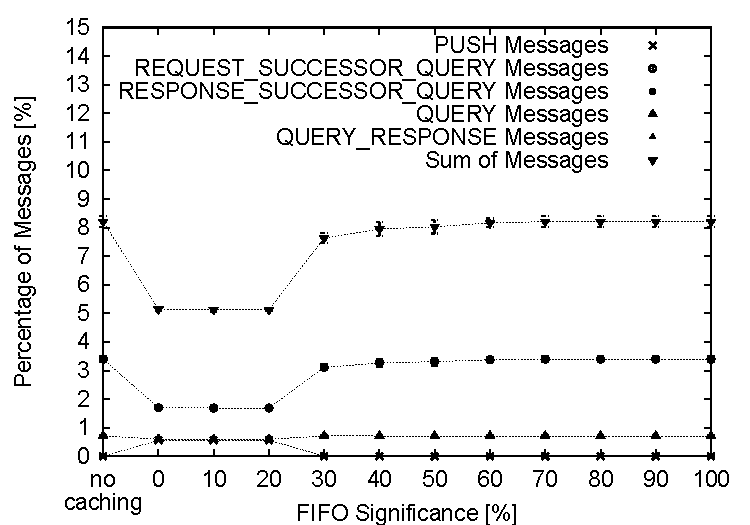
\includegraphics[width=0.48\linewidth]{pic4}}
 \caption[Observed message fractions and 95\% confidence intervals for Chord]{Observed message fractions and 95\% confidence intervals for Chord without the influence of churn. The FIFO capacity varies from 20 (\ref{fig:multipic:a}) -- 50 (\ref{fig:multipic:d}) entries (decadic steps).}
 \label{fig:multipic} %% label for entire figure
\end{figure}

\subsection{Programm Code}
Eine elegante M�glichkeit, Programmtext einzubinden, l�sst sich mit dem listings-Paket erreichen.
Das \verb|HelloWorld| Programm aus Listing \ref{lst:hw} hat in Zeile \ref{line:hw3} �brigens einen Programmierfehler.
\begin{lstlisting}[float=htp,caption=Hello World,label=lst:hw,language=Java, numbers=left, numberstyle=\tiny, stepnumber=2, numbersep=8pt, escapeinside={//@}{@//},backgroundcolor=\color{yellow},xleftmargin=3ex,xrightmargin=1ex]
public class HelloWorld {
    public static void main(String[] args) {
        Syste.out.println("Hello, World"); //@\label{line:hw3}@//
    }
}
\end{lstlisting}

\subsection{Fu�noten}
Wenn man auf Google \footnote{\url{http://www.google.com}} verweisen will, bietet sich statt einer gesonderten
Referenz auch einfach eine Fu�note an.
\subsection{Formeln}
Man kann mit \LaTeX\ sehr sch�n Formeln erzeugen:
$$L_{P}(k) = R^{orig}_{P}(k) + \sum_{i=0}^n 2*R^{i}_{P}(k)$$

    \chapter{Einleitung}\label{sec:Introduction}
%\section{Erstes Unterkapitel}
%\subsection{Quellenangaben}\label{subsec:sources}
Wir zitieren hier die Quellen \cite{Agarwal2006}, \cite{Ahlgren2012}, \cite{Bayardo2007}, \cite{Broder2004}, \cite{Byers2002}, \cite{Duerr2010}, \cite{Hellerstein1994}, \cite{Lehman1986}, \cite{Mitzenmacher2002}, \cite{Nafe2005}, \cite{Qiao2014}, \cite{Ruppel2014}, \cite{Sakuma2011}, \cite{Sarwat2012}, \cite{Schnell2013}, \cite{Schoenfeld2014}, \cite{Shiraki2009}, \cite{Werner2015}, \cite{Yang2002}, \cite{Zhang2012}, \cite{Zhu2004}, die in der Datei\\
\verb|bibliography.bib|
stehen.
%\subsection{Referenz auf anderen Text}
%Es ist auch möglich auf andere Stellen im Text z.B. Kapitel \ref{subsec:sources} zu verweisen.
%\subsection{Tabellen}
%Es gibt schöne Möglichkeiten Tabellen einzubinden wie z.B. Tabelle \ref{tab:CommonParameterSettings}.
%\begin{center}
%\begin{table}[htbp]
%{\small
%\begin{center}
%\begin{tabular}[center]{lrlc}
%\toprule
%Parameter & Value & (Unit) & Available for Chord \\
%\midrule
%Query timeout & 10 & seconds & $\surd$ \\
%Republish timeout & 300 & seconds & $\surd$ \\ % explain this value...
%Stabilize timeout & 5 & seconds & $\surd$ \\
%Fix fingers timeout & 30 & seconds & $\surd$ \\
%Message timeout & 1 & second & $\surd$ \\
%Connect timeout & 10 & seconds & $\surd$ \\
%Ping superpeer timeout & 5 & seconds & $\times$ \\
%Cost-Optimality estimation timeout & 20 & seconds & $\times$ \\
%Significance for change in number of superpeers & 10 & percent & $\times$ \\
%Significance for change in estimations  & 10 & percent & $\times$ \\
%Number of permanent superpeers & 32 & nodes & $\times$ \\
%Mean number of peers & 1000 & nodes & $\surd$ \\
%Mean number of lookups per hour & 60 & queries & $\surd$ \\
%Mean number of shared InfoProfiles per node & 20 & & $\surd$ \\
%Identifier space & 16 & bits & $\surd$ \\
%Direct insertion acknowledgment & true & bool & $\times$ \\
%Direct query responses & true & bool & $\times$ \\
%Force query resolution & true & bool & $\surd$  \\
%\bottomrule
%\end{tabular}
%\end{center}
%} % end of tiny
%\caption[Simulation parameter settings]{Common simulation parameter settings.\label{tab:CommonParameterSettings}}
%\end{table}
%\end{center}
%
%\subsection{Bilder}
%Man kann sehr einfach Bilder einbinden so wie z.B. in Abbildung \ref{fig:pic0}.
%\begin{figure}[hpbt]
%  \centering
%  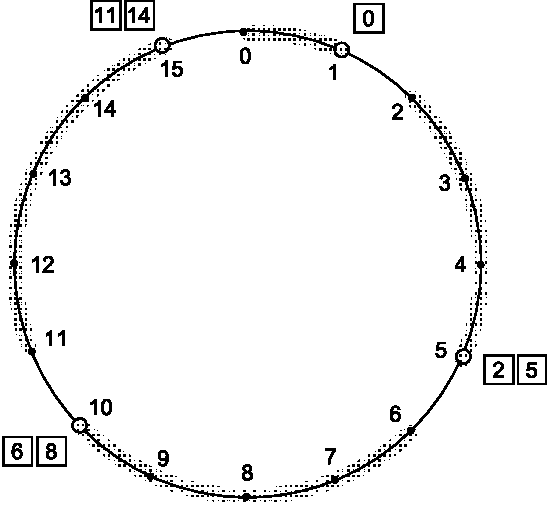
\includegraphics[width=0.4\textwidth]{pictures/pic0}\\
%  \caption[Example of a $4$-bit Chord identifier circle]{Example of a $4$-bit Chord identifier circle.
%  The responsibility ranges for each peer are accentuated in light gray}\label{fig:pic0}
%\end{figure}
%Es lassen sich auch mehrere Bilder nebeneinander platzieren wie z.B. in Abbildung
%\ref{fig:multipic} zu sehen ist.
%\begin{figure}[hpbt]
% \centering
%  %%----start of first subfigure----
%  \subfloat[FIFO size limited to 20 entries]{
%   \label{fig:multipic:a} %% label for first subfigure
%   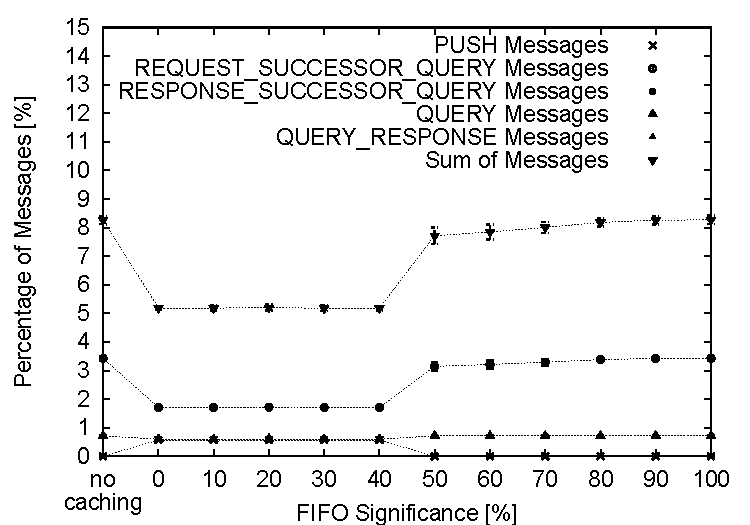
\includegraphics[width=0.48\linewidth]{pic1}}
%  \hspace{0.01\textwidth}
%  %%----start of second subfigure----
%  \subfloat[FIFO size limited to 30 entries]{
%   \label{fig:multipic:b} %% label for second subfigure
%   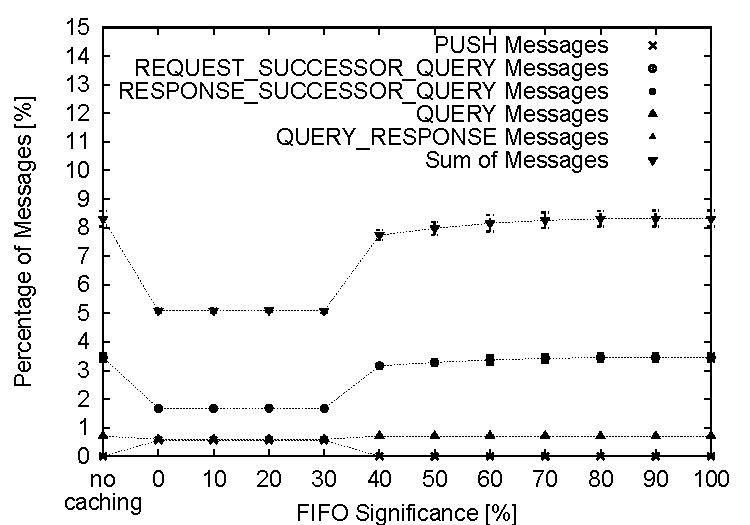
\includegraphics[width=0.48\linewidth]{pic2}}\\[0pt] % horizontal break
%  %%----start of third subfigure----
%  \subfloat[FIFO size limited to 40 entries]{
%   \label{fig:multipic:c} %% label for third subfigure
%   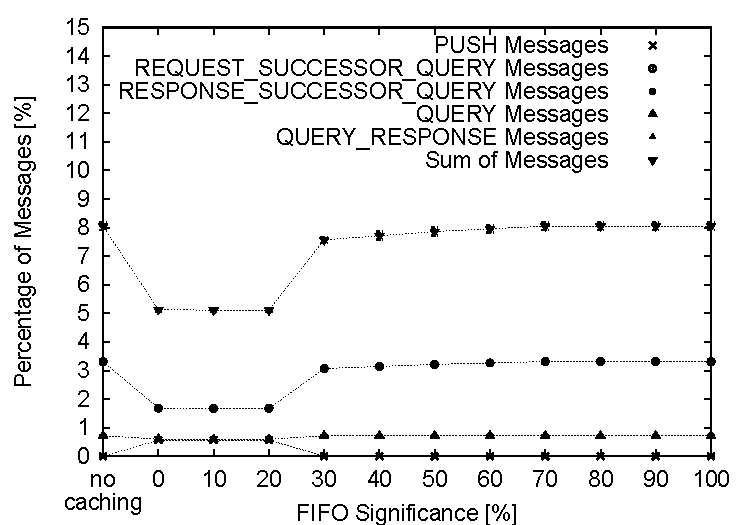
\includegraphics[width=0.48\linewidth]{pic3}}
%  \hspace{0.01\textwidth}
%  %%----start of fourth subfigure----
%  \subfloat[FIFO size limited to 50 entries]{
%   \label{fig:multipic:d} %% label for fourth subfigure
%   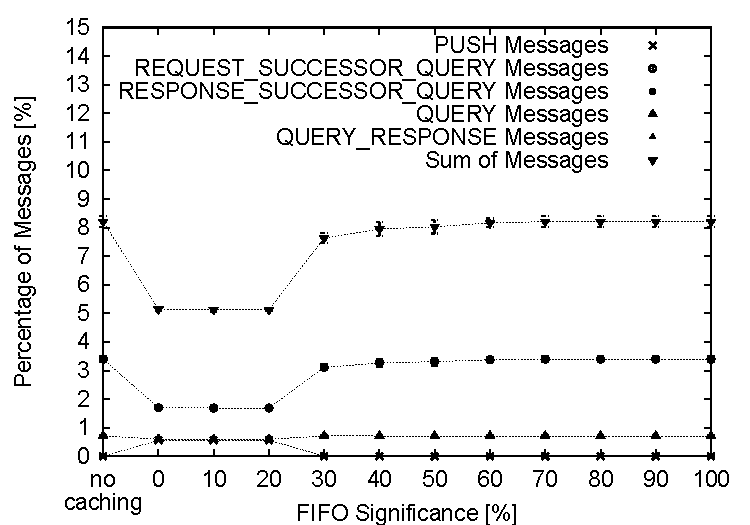
\includegraphics[width=0.48\linewidth]{pic4}}
% \caption[Observed message fractions and 95\% confidence intervals for Chord]{Observed message fractions and 95\% confidence intervals for Chord without the influence of churn. The FIFO capacity varies from 20 (\ref{fig:multipic:a}) -- 50 (\ref{fig:multipic:d}) entries (decadic steps).}
% \label{fig:multipic} %% label for entire figure
%\end{figure}
%
%\subsection{Programm Code}
%Eine elegante Möglichkeit, Programmtext einzubinden, lässt sich mit dem listings-Paket erreichen.
%Das \verb|HelloWorld| Programm aus Listing \ref{lst:hw} hat in Zeile \ref{line:hw3} übrigens einen Programmierfehler.
%\begin{lstlisting}[float=htp,caption=Hello World,label=lst:hw,language=Java, numbers=left, numberstyle=\tiny, stepnumber=2, numbersep=8pt, escapeinside={//@}{@//},backgroundcolor=\color{yellow},xleftmargin=3ex,xrightmargin=1ex]
%public class HelloWorld {
%    public static void main(String[] args) {
%        Syste.out.println("Hello, World"); //@\label{line:hw3}@//
%    }
%}
%\end{lstlisting}
    % further chapters
%
% =================================================================================================
% place your appendix here
% -------------------------------------------------------------------------------------------------
%
    \appendix
    % % -------------------------------------------------------------------------------------------------
%      MDSG Latex Framework
%      ============================================================================================
%      File:                  appendix.tex
%      Author(s):             Michael Duerr
%      Version:               1
%      Creation Date:         30. Mai 2010
%      Creation Date:         30. Mai 2010
%
%      Notes:                 - Place your appendix here
%                             - Use the same commands (`chapter', `section', ...) as in main text
% -------------------------------------------------------------------------------------------------
%
\chapter{Anhang}\label{ch:anhang}
\section{Die Klasse \texttt{BloomFilterTree}}\label{sec:BloomFilterTree.hpp}
\small{
\begin{verbatim}
//  BloomFilterTree.hpp, Judith Greif
//  Description: Header for class BloomFilterTree

#ifndef BloomFilterTree_hpp
#define BloomFilterTree_hpp

#include "BloomFilterNode.hpp"
#include "BloomFilterIndexNode.hpp"
#include "BloomFilterLeaf.hpp"

using namespace std;

class BloomFilterTree {
    
private:
    int t;                          // Order = minimum degree
    int filtersize;                 // Size of associated Bloom filters (# of bits)
    
public:
    BloomFilterNode *root;          // Pointer to root node   
    BloomFilterTree(int _t, int _s);
    ~BloomFilterTree();   
    BloomFilterNode *getRoot();
    
    // Tree management
    void traverse();
    void traverseFilters();
    double computeMinJaccard(BloomFilter *filter);
    double computeMaxJaccard(BloomFilter *filter);
    int getMinJaccardKey(BloomFilter *filter);
    BloomFilter *getMinJaccardFilter(BloomFilter *filter);
    int getMinKey();
    int getMaxKey();
    vector<BloomFilter> collectAllFilters();
    int countFilters();
    int countUnionFilters(); 
    int computeSubsetId(BloomFilter *filter);
    int computeSupersetId(BloomFilter *filter);
    bool contains(int k);
    BloomFilterNode *search(int k);
    vector<pair<int, double>>computeAllDistances(BloomFilter *filter);
    vector<pair<int, double>>computekDistances(BloomFilter *filter, int k);
    int countLeaves(); 
    
    // Measurement and comparison
    vector<pair<BloomFilter, double>> compare(BloomFilter *filter, int k);
    vector<int> compareMem();
    vector<double> compareConstrCost();
    vector<int> compareComplSimQuery(BloomFilter *filter);
    vector<int> compareComplSimQueryVec(BloomFilter *filter, int k);
    
    // Insertion
    void insert(BloomFilter *filter);
    void insertAsSets(BloomFilter *filter);
    
    // Similarity queries
    BloomFilter *simQuery(BloomFilter *filter);
    vector<BloomFilter*> simQueryVec(BloomFilter *filter, int k);
};

#endif
\end{verbatim}
}
\newpage
\section{Die Klasse \texttt{BloomFilter}}\label{sec:BloomFilter.hpp}
\small{
\begin{verbatim}
//  BloomFilter.hpp, Judith Greif
//  Description: Header for class BloomFilter

#ifndef BloomFilter_hpp
#define BloomFilter_hpp

#include <iostream>
#include <vector>
#include <cstdlib>
#include <random>
#include <math.h>
#include <string>
#include <functional>

using namespace std;

const int NUM_FILTERS = 100;
const int NUM_ELEMENTS = 50;
const int NUM_QUERYFILTERS = 10;
const int seed = rand();

class BloomFilter {
    
private:
    int id;
    int count;                  // # of elements inserted
    int size;                   // # of bits
    int d;                      // # of hash functions
    int *data;
    
public:
    BloomFilter();
    BloomFilter(const BloomFilter& fSource);
    BloomFilter(int _id, int _size);
    ~BloomFilter();   
    BloomFilter & operator = (const BloomFilter &fSource);   
    void setId(int value);
    int getId();
    int getSize();
    void setValue(int index, int value);
    int *getData();   
    void printData();
    void printArr();
    void initRandom();
    double fractionOfZeros();
    double eSize();
    BloomFilter *logicalOr(BloomFilter *filter);
    BloomFilter *logicalAnd(BloomFilter *filter);
    bool isSubset(BloomFilter *filter);
    bool isSuperset(BloomFilter *filter);
    int mySupersetCount();
    int mySubsetCount();
    int binomialCoefficient(int n, int k);
    int setOnes();
    int setZeros();
    int validOnes();
    int possibleFreeZeros();
    int possibleAddedOnes();
    double setUnion(BloomFilter *filter) const;
    double setIntersection(BloomFilter *filter) const;
    double computeAmbienceJaccard(BloomFilter *filter);
    double computeJaccard(BloomFilter *filter) const;
    double eUnion(BloomFilter *filter);
    double eIntersect(BloomFilter *filter);
    void add(string &elem);
    void increment();
    int getNumHashes();
    bool checkCorrectFillDegree();
};

#endif
\end{verbatim}
\newpage
\section{Die Methode \texttt{computeSubsetId()} der Klasse \texttt{BloomFilterLeaf()}}\label{sec:computeSubsetId()}
\small{
\begin{verbatim}
int BloomFilterLeaf::computeSubsetId(BloomFilter *filter) {
    vector<pair<int, double>> subsets;
    vector<int> freeIds;
    vector<pair<int, int>> goodIds;
    BloomFilterLeaf *tmp = this;
    double jacc;
    int minId = filters[0]->getId()-1;
    int maxId;
    int optId;
    bool no_subsets = true;
    while (tmp != NULL) {
        
        // Collect all filters that filter is subset of
        for (int i=0; i<tmp->getCount(); i++) {
            if ((tmp->filters[i])->isSubset(filter)) {
                jacc = computeJaccard(tmp->filters[i], filter);
                subsets.push_back(make_pair(tmp->filters[i]->getId(), jacc));
                no_subsets = false;
            }
        }
        maxId = tmp->filters[tmp->getCount()-1]->getId()+1;
        tmp = tmp->getNext();
    }
    
    // Sort subsets by jacc distances in ascending order
    sort(subsets.begin(), subsets.end(), [](const pair<int, double> &left, 
    const pair<int, double> &right) {
        return left.second < right.second;
    });
    
    // Collect free ids
    tmp = this;
    freeIds.push_back(minId);
    freeIds.push_back(maxId);
    while (tmp != NULL) {
        for (int i=0; i<tmp->getCount()-2; i++) {
            for (int j=tmp->filters[i]->getId()+1; j<tmp->filters[i+1]->getId(); j++) {
                if (j<tmp->filters[i+1]->getId()) {
                    freeIds.push_back(j);
                }
            }
            if (tmp->getCount() < tmp->getMax()) {
                if (tmp->getNext() != NULL) {
                    int start = tmp->filters[tmp->getCount()-1]->getId()+1;
                    int last = tmp->getNext()->filters[0]->getId();
                    for (int j=start; j<last; j++) {
                        freeIds.push_back(j);
                    }
                }
            }
            
        }
        tmp = tmp->getNext();
    }
    sort(freeIds.begin(), freeIds.end(), less<int>());
    
    // If there are no subsets, return smallest free id as pair with numerical distance 0
    if (no_subsets == false) {
        
        // Determine optimal id
        // Check subsets in ascending order
        // Get next greater and smaller id
        int distNeg = subsets[0].first - minId;
        int distPos = maxId - subsets[0].first;
        for (int i=0; i<subsets.size(); i++) {
            optId = subsets[i].first;
            int j=0;
            while (freeIds[j] < subsets[i].first) {
                if (optId-freeIds[j] < optId-minId) {
                    minId = freeIds[j];
                    distNeg = optId-minId;
                }
                j++;
            }
            
            j=freeIds.size()-1;
            while (freeIds[j] > subsets[i].first) {
                if (freeIds[j]-optId < maxId-optId) {
                    maxId = freeIds[j];
                    distPos = maxId-optId;
                }
                j--;
            }
            goodIds.push_back(make_pair(minId, distNeg));
            goodIds.push_back(make_pair(maxId, distPos));
        }
        
        // Sort next smaller and greater ids by numerical distance in ascending order
        sort(goodIds.begin(), goodIds.end(), [](const pair<int, int> &left, 
        const pair<int, int> &right) {
            return left.second < right.second;
        });
    }
    else {
        goodIds.push_back(make_pair(freeIds[0], 0));
    }
    
    // Return first element
    return goodIds[0].first;
}
\end{verbatim}
}
    % further appendix
%
% =================================================================================================
% comment \listoffigures and/or \listoftables if not wanted
% -------------------------------------------------------------------------------------------------
%
    \backmatter
    % \listoffigures                                % list of figures (uncomment if wanted)
    % \listoftables                                 % list of tables (uncomment if wanted)
    % \lstlistoflistings                            % list of listings (uncomment if wanted)
%
% =================================================================================================
% place your bibliography here
% -------------------------------------------------------------------------------------------------
%
    \begin{spacing}{0.9}                          % save some space
    	   %\nocite{*}
       %\bibliographystyle{geralpha}               % for german thesis
       \bibliographystyle{alpha}                 % for english thesis
       \bibliography{bibliography}                % the location of bib file
    \end{spacing}
\end{document}
%
% =================================================================================================
% end of document
% -------------------------------------------------------------------------------------------------
%
